\documentclass[11pt]{article}
\usepackage[utf8]{inputenc}
\usepackage{amsmath}
\usepackage{amsfonts}
\usepackage{amssymb}
\usepackage{graphicx}
\usepackage[super]{nth}
\usepackage{amsthm}
\usepackage{bm}
\newtheorem{theorem}{Theorem}
\newtheorem{objective}{Objective}
\newtheorem{model}{Model}
\usepackage{xcolor}
\definecolor{light-gray}{gray}{0.95}
\newcommand{\code}[1]{\colorbox{light-gray}{\texttt{#1}}}
\usepackage{listings}

\usepackage[authoryear]{natbib}


\makeatletter
\renewcommand{\maketitle}{
\begin{center}

\pagestyle{empty}

{\Large \bf \@title\par}
\vspace{1cm}

{\LARGE Marcel Gietzmann-Sanders}\\[1cm]

STAT641 - Bayesian Statistics \\
University of Alaska Fairbanks


\end{center}
}\makeatother


\title{Implementing a BYM Model in Stan to Fit Boston Housing Price Data}

\date{2024}
\setcounter{tocdepth}{2}
\begin{document}
\maketitle

\section{Data on Boston Housing Prices in 1978}

For this study we'll be using a dataset originally published in 1978 on housing prices in Boston, Massachusetts (\cite{origin}). This data was made accessible through \code{spData} package in R (\cite{spdata}). Specifically this dataset contains median house prices and potential covariates for 506 tracts in the Greater Boston Area. Fig. \ref{fig:prices} shows the median price per tract of land where it should be understood that this data is censored and median values over \$50,000 are capped. A full list of covariates can be found in the documentation for the \code{boston} dataset in \code{spData}. What we wish to understand is which of these covariates are indeed related to housing prices after being added to a spatial bayesian model. \newline

\begin{figure}[h!] 
  \centering
  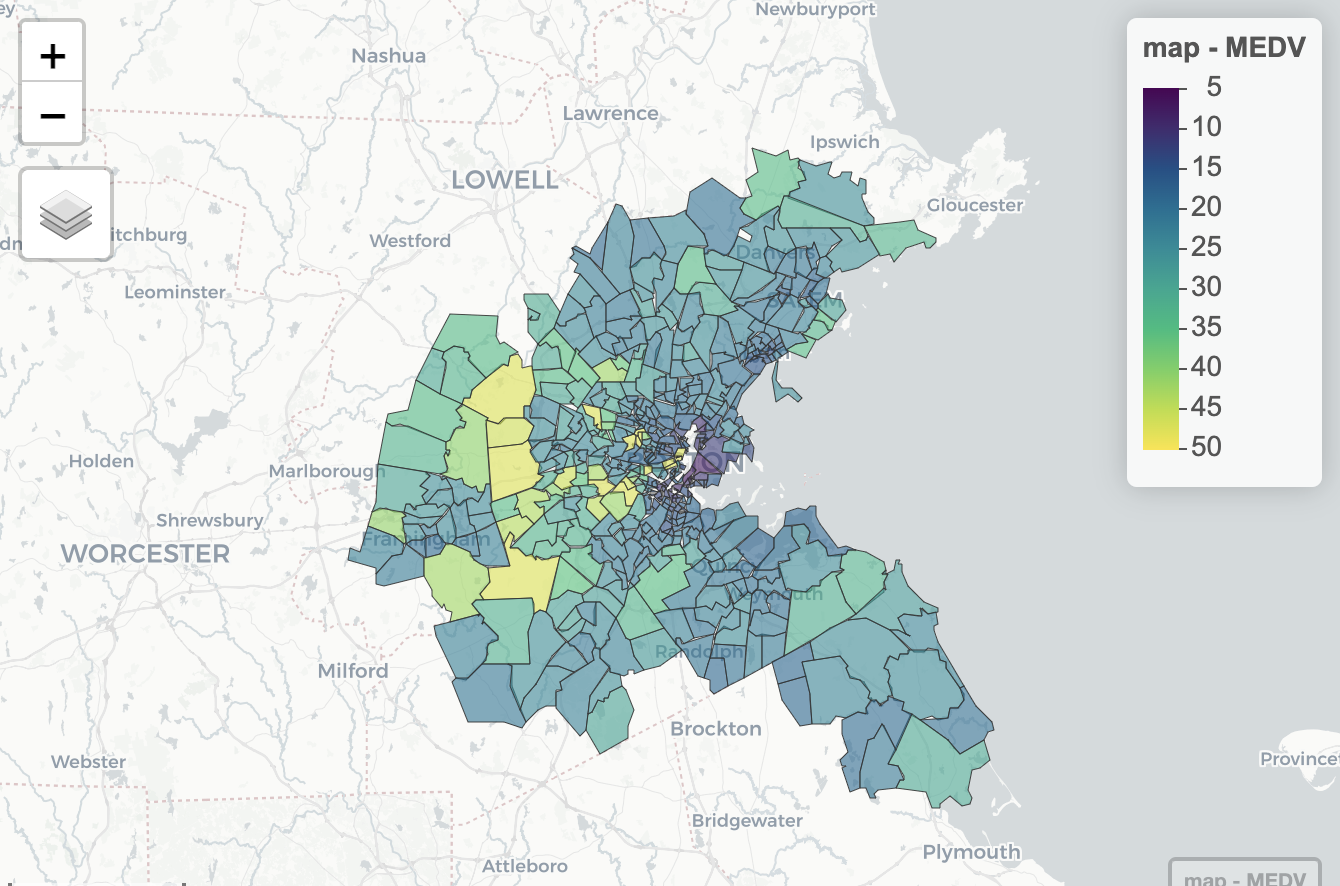
\includegraphics[height=75mm]{prices.png}
  \caption{Median Housing Price}
  \medskip
	\small
	The median house value (in \$1000USD) by census tract in the Greater Boston Area.
  \label{fig:prices}
\end{figure}

Starting with some exploratory data analysis we identified four covariates of particular interest. Crime rates per capita, average number of rooms per dwelling, weighted distance to employment centers, and the nitric oxide concentrations per town. 

First, as the distribution of values is right skewed (and following in the footsteps of (\cite{book})) we took as our target variable the logarithm of the median house value per tract instead of the median value itself. Fig. \ref{fig:price_dist} shows the distribution of our target. 

\begin{figure}[h!] 
  \centering
  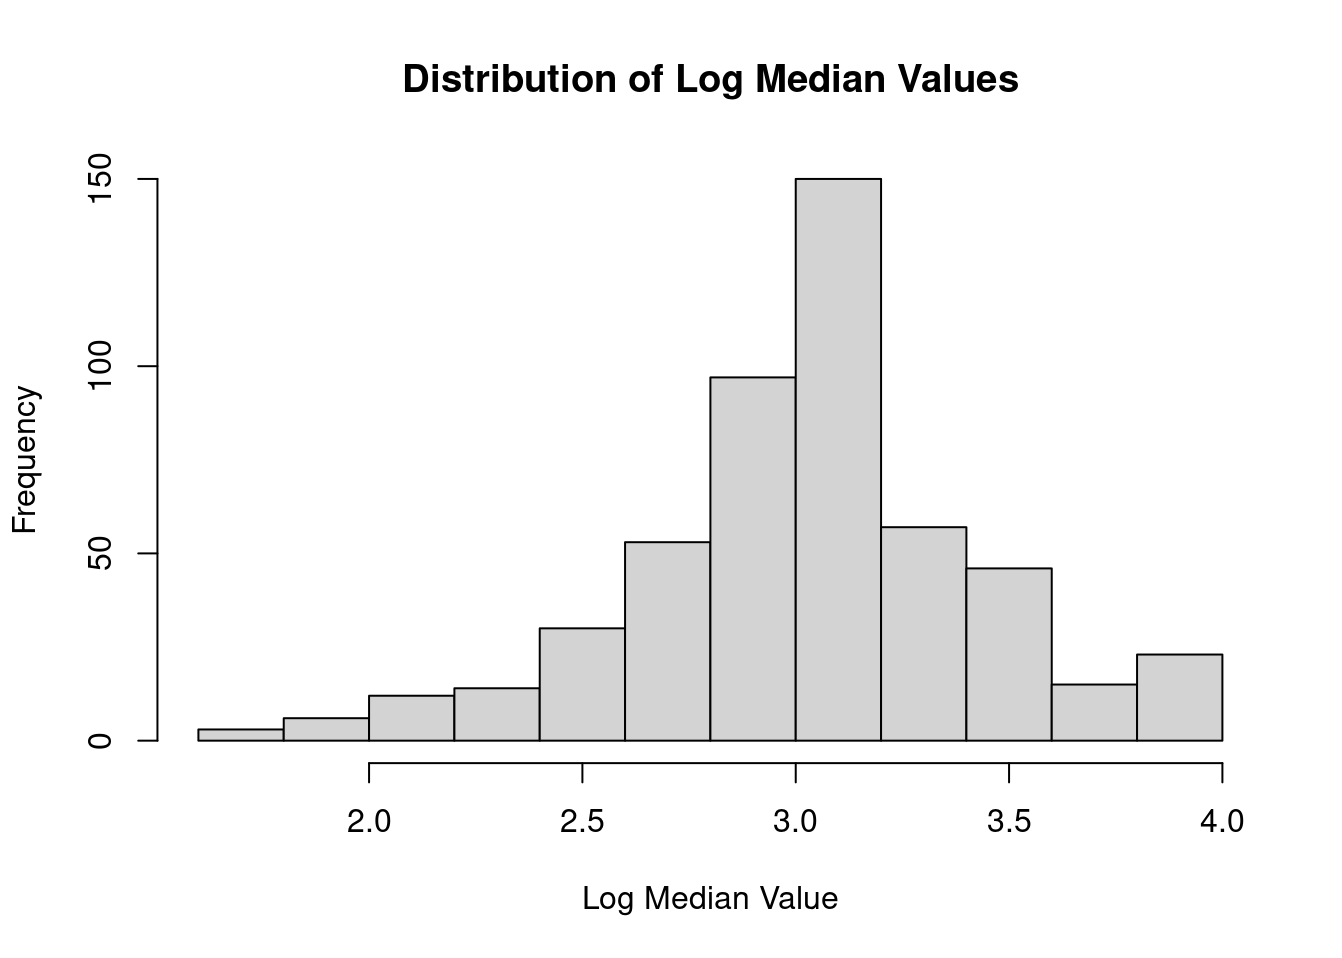
\includegraphics[height=75mm]{price_dist.png}
  \caption{Log Median Housing Price Distribution}
  \label{fig:price_dist}
\end{figure}

Fig. \ref{fig:crime} shows the relationship between per capita crime rate and our target with a clear negatively correlated relationship between then two and a rather wide spread of values in and around 0. 

Fig. \ref{fig:rooms} shows how our target varies with the average number of rooms per dwelling in each tract. Here we can see a strong positive relationship between the two which makes a great deal of sense. 

In Fig. \ref{fig:employment} we see a similar positive relationship between the logarithm of the average weighted distance to employment centers and our target. However this relationship is not as clear or strong as the one between our target and the number of rooms per dwelling. 

Finally Fig. \ref{fig:nox} shows us the relationship between nitric oxide concentrations in parts per million and our target with a somewhat spurious negative relationship. 

\begin{figure}[h!] 
  \centering
  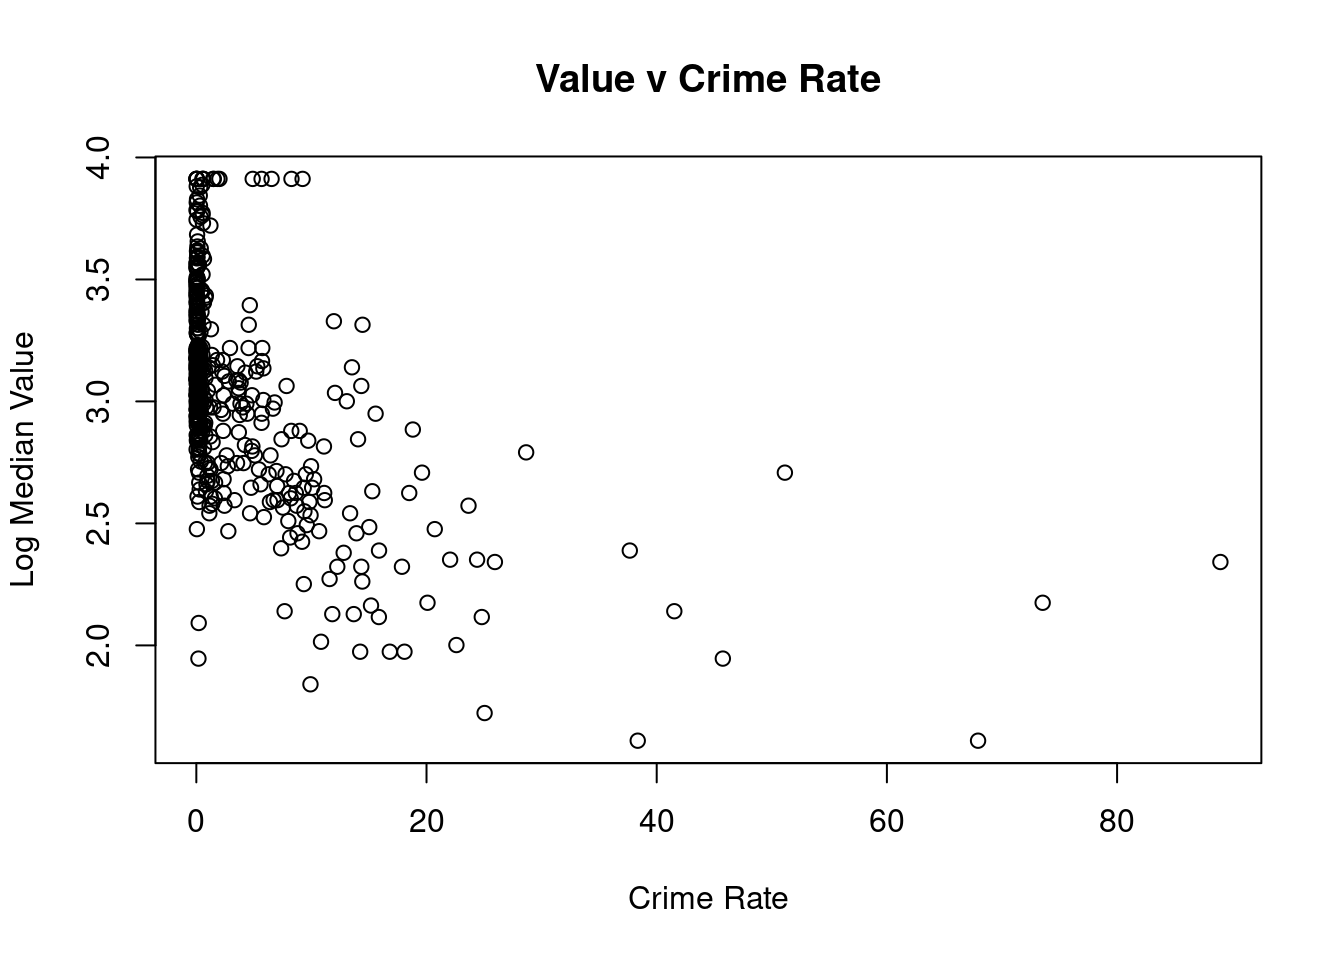
\includegraphics[height=75mm]{crime.png}
  \caption{Log Median Price vs Crime Rate}
  \label{fig:crime}
\end{figure}

\begin{figure}[h!] 
  \centering
  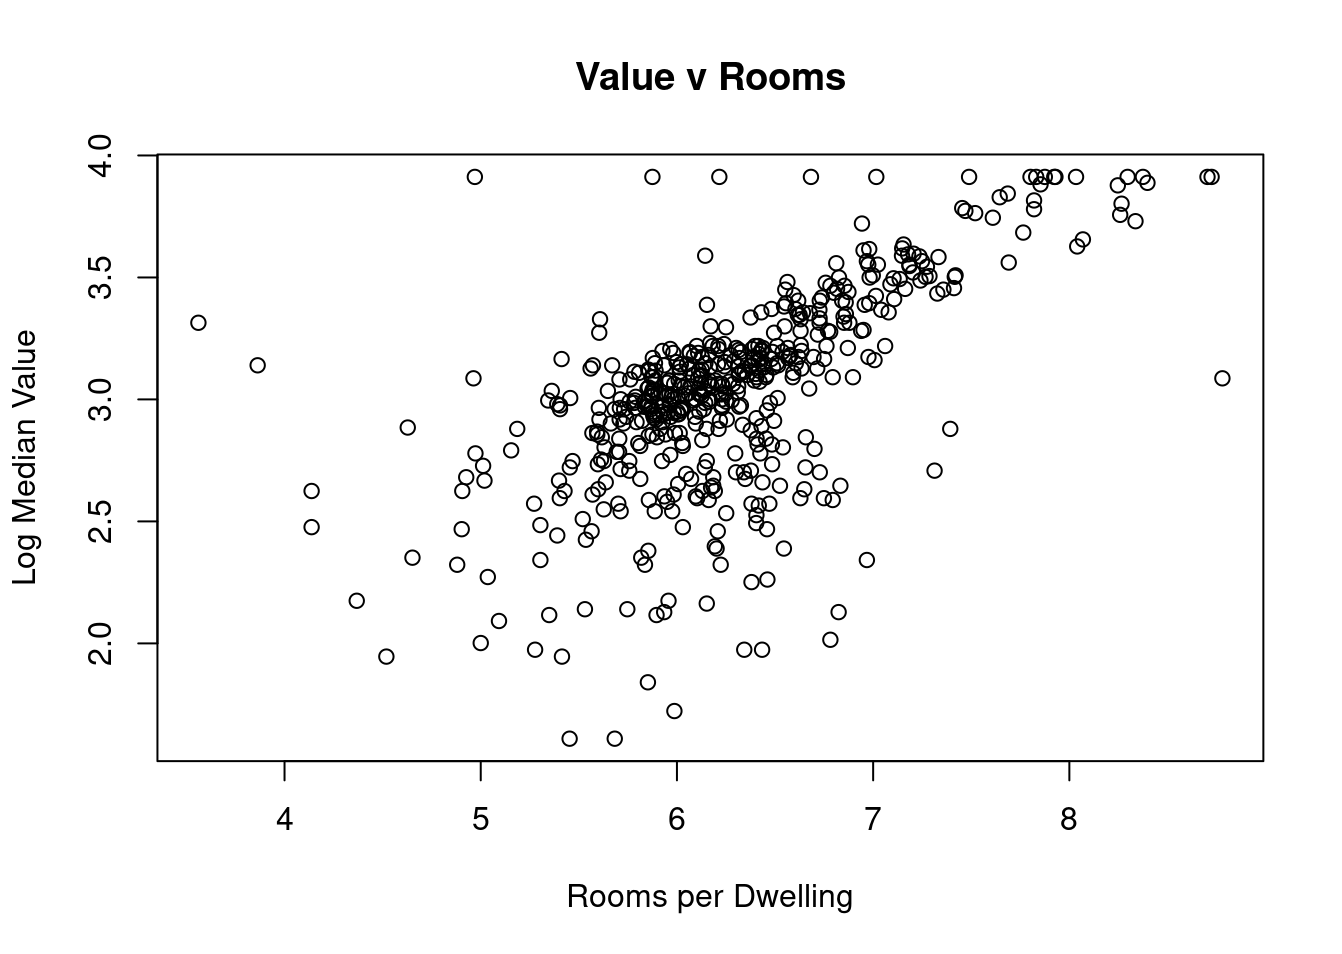
\includegraphics[height=75mm]{rooms.png}
  \caption{Log Median Price vs Rooms per Dwelling}
  \label{fig:rooms}
\end{figure}

\begin{figure}[h!] 
  \centering
  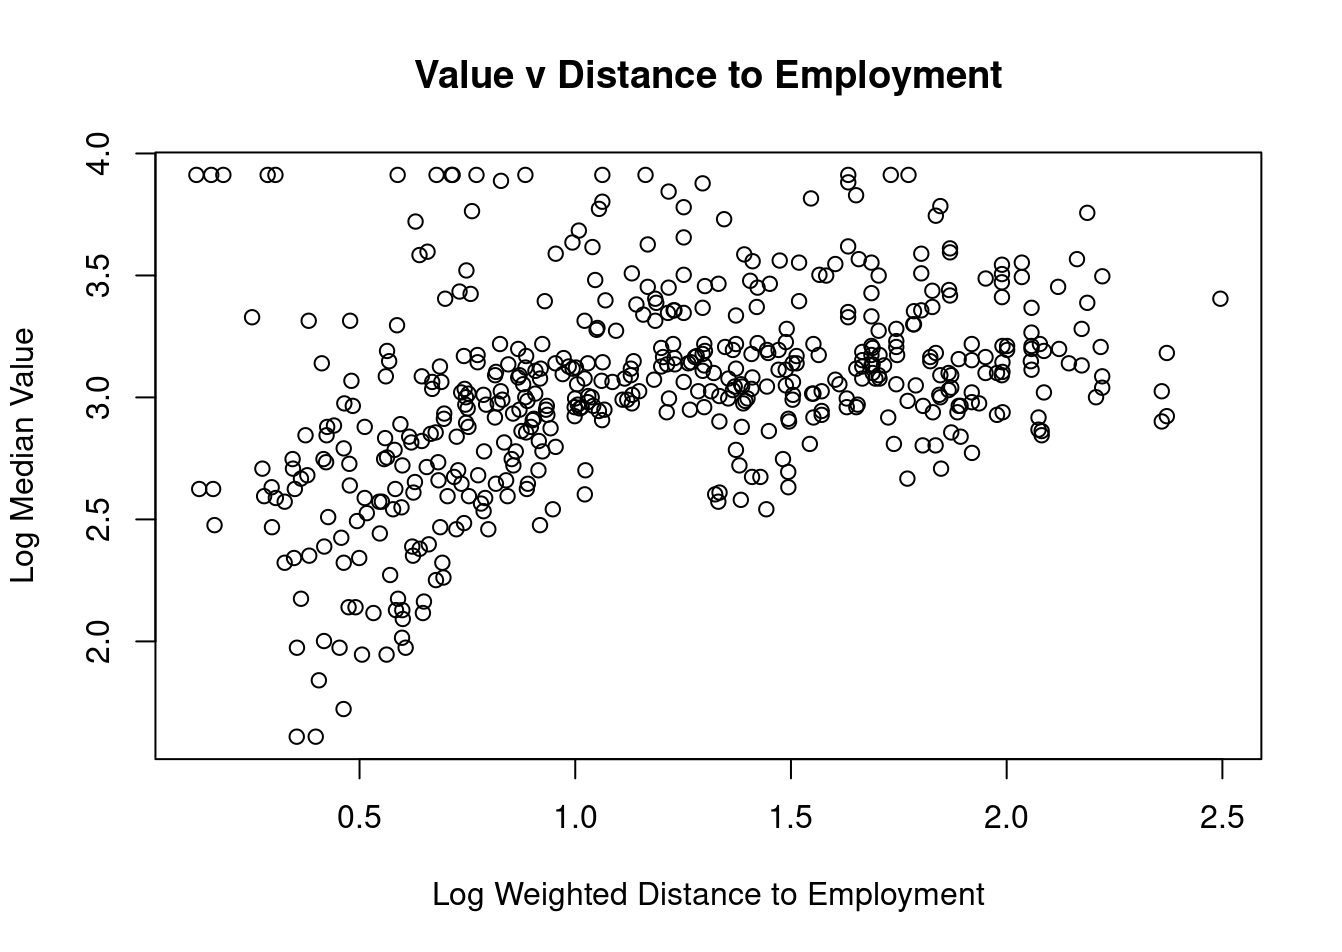
\includegraphics[height=75mm]{employment.png}
  \caption{Log Median Price vs Log Weighted Distance to Employment Centers}
  \label{fig:employment}
\end{figure}

\begin{figure}[h!] 
	\centering
  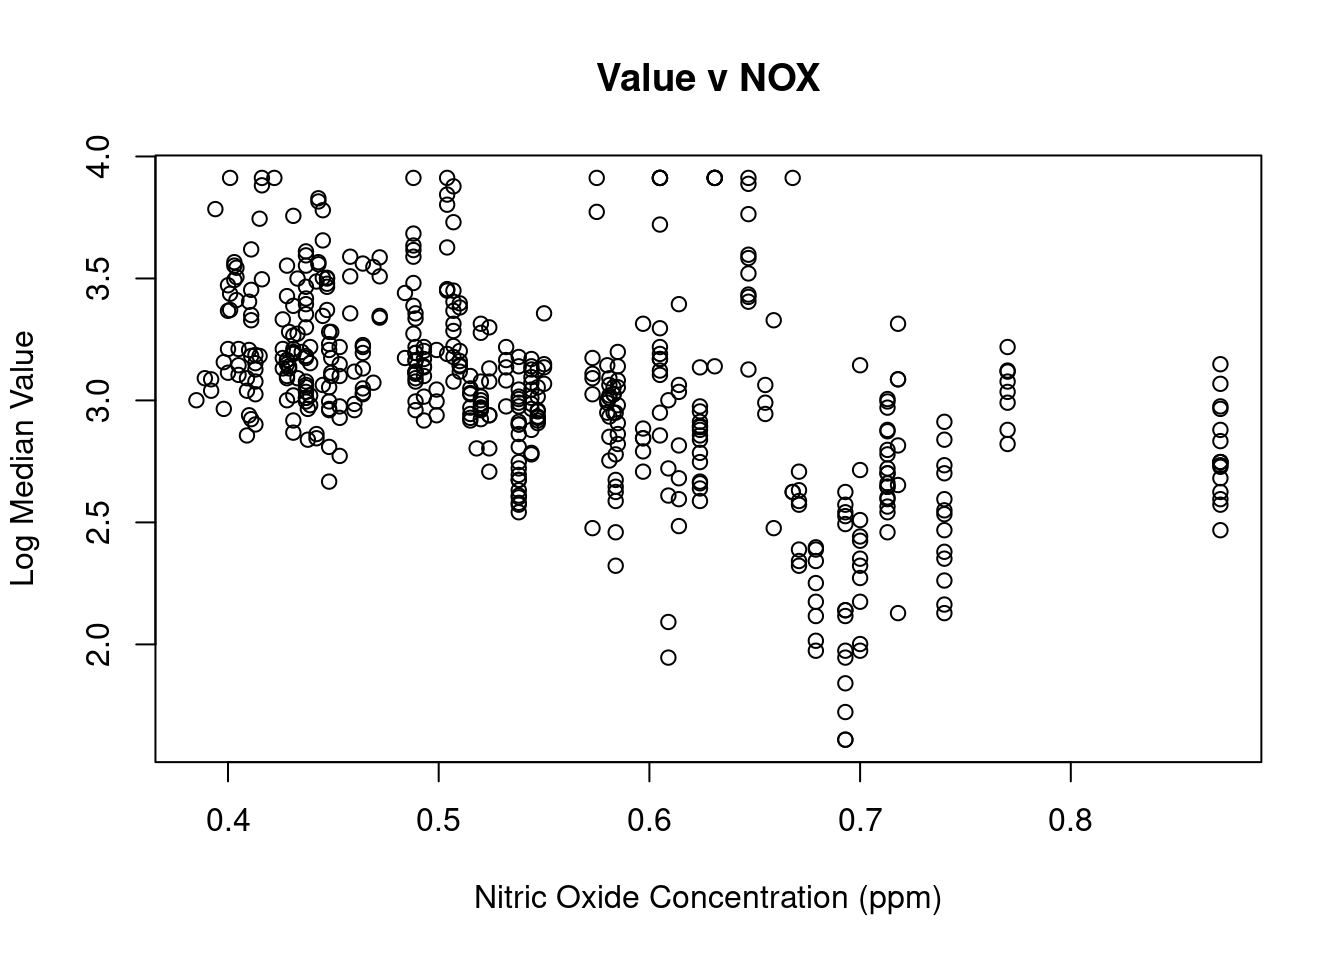
\includegraphics[height=75mm]{nox.png}
  \caption{Log Median Price vs NOX}
  \label{fig:nox}
\end{figure}

\section{Defining the Model}

We will be using a variant of the Besag-York-Mollié (BYM) model (\cite{book})(\cite{bymstan}). In this model we assume that we have a series of $Y_i$ which is a vector of our target variable (log median housing value in our case) for each tract $i$. Furthermore we assume our $Y_i$ can be modeled as a normal distribution:

$$Y_i \sim Normal(\mu_i, \sigma^2)$$

where it is the $\mu_i$ that will be affected by our covariates. Specifically we will have:

$$\mu_i= \beta_0 + \vec{\beta} \vec{x_i} + \sigma_r\left( \sqrt{\rho}\phi_i + \sqrt{1-\rho}\theta_i \right)$$

where $\beta_0$ is our intercept, $\vec{\beta}$ are the coefficients for our models effects from each covariate, $x_i$ are our covariates corresponding to tract $i$, $\phi_i$ and $\theta_i$ are spatial and random effects respectively, and $sigma_r$ and $\rho$ allow us to control the effect of the random variables as well as the degree to which our model has spatial and/or unstructured noise (if $\rho=1$ we have only spatial structure whereas if $\rho=0$ it is totally unstructured). 

For our more straightforward priors we will have:

$$\beta_0 \sim Normal(0,1)$$
$$\beta_i \sim Normal(0,1)$$
$$\theta_i \sim Normal(0,1)$$
$$\sigma \sim Normal(0,1)$$
$$\sigma_r \sim Normal(0,1)$$
$$\rho = \frac{e^{r}}{1 + e^{r}}, r\sim Normal(0,1)$$

Our spatial terms $\phi_i$ are a little more complicated. \newline

Each spatial interaction term $\phi_i$ is modeled as conditional on the other terms as:

$$\phi_i | \phi_j \sim N\left(\sum_j w_{ij}\phi_j, \sigma^2  \right), i\neq j$$

the name of which is a conditional autoregressive model (CAR). A key result that Besag proved (\cite{besag}) is that the joint distribution $\bm{\phi}$ ends up being multivariate normal random variable centered at 0

$$\vec{\phi}\sim N(0, Q^{-1})$$

where $Q=D(I-\alpha A)$ where $D$ is a diagonal "neighbors" matrix (each element on the diagonal is the number of neighbors unit $i$ has), $A$ is an adjacency matrix where if $i,j$ are neighbors then the $i,j$ element is 1, and $\alpha$ lets us control spatial dependence. This results in a log probability density of $\vec{\phi}$ which is proportional to:

$$\frac{n}{2}\log{(\det{Q})}-\frac{1}{2}\vec{\phi}^T Q \vec{\phi}$$

Given $\det{Q}$ is a constant and MCMC samplers compute the log probability up to a proportionality constant (\cite{bymstan}) the first term drops out of the computation thereby reducing the computational intensity of this evaluation. 

In our case, as we will be following the stan implementation from the paper (\cite{bymstan}) we will be setting $\alpha=1$ and thereby get an intrinsic conditional autoregressive model (ICAR) which reduces $Q$ to $D-A$. With an ICAR model each $\phi_i$ is distributed with a mean equal to the average of its neighbors. If we additionally assume that $\vec{\phi}$ is centered at zero with common variance 1, then the joint probability of $\vec{\phi}$ becomes (\cite{bymstan}):

$$p(\vec{\phi})\propto \exp{\left( -\frac{1}{2} \sum_{i\sim j} (\phi_i - \phi_j)^2 \right)}$$

where $i \sim j$ indicates that $i$ and $j$ are neighbors. This then is our prior for the $\phi_i$ - an ICAR model centered at $0$ with common variance $1$. 

\section{Implementing the Model}

Here we have the \code{stan} model itself:

\begin{lstlisting}[language=C++, basicstyle=\small]

functions {
    real icar_normal_lpdf(vector phi, int N, int[] node1, int[] node2) {
        return -0.5 * dot_self(phi[node1] - phi[node2]) 
            + normal_lpdf(sum(phi) | 0, 0.001 * N);
    }
}
data {
    int<lower=0> N; // number of tracts
    int<lower=0> N_edges; // number of unique edges
    int<lower=1, upper=N> node1[N_edges]; // start of edge
    int<lower=1, upper=N> node2[N_edges]; // end of edge
    int<lower=1> K; // number of covariates
    matrix[N, K] x; // design matrix
    real y[N]; // target
}
parameters {
    real beta0;
    vector[K] betas;

    real<lower=0> sigma;
    real logit_rho;

    vector[N] phi;
    vector[N] theta;

    real<lower=0> sigma_r;
}
transformed parameters {
    real<lower=0, upper=1> rho = inv_logit(logit_rho);
    vector[N] convolved_re = sqrt(rho) * phi 
                                + sqrt(1 - rho) * theta;
}
model {
    y ~ normal(beta0 + x * betas + convolved_re * sigma_r, sigma);
    target += icar_normal_lpdf(phi | N, node1, node2);
    beta0 ~ normal(0, 1);
    betas ~ normal(0, 1);
    logit_rho ~ normal(0, 1);
    sigma ~ normal(0, 1);
    theta ~ normal(0, 1);
    sigma_r ~ normal(0, 1);
}

\end{lstlisting}

Note the term \verb+normal_lpdf(sum(phi)|0,0.001*N)+ used to center $\vec{\phi}$ at zero (\cite{bymstan}). 

\section{Fitting the Model}

First we need to setup all of our data:

\begin{lstlisting}[language=R, basicstyle=\small]
library(sf)
library(spData)
library(mapview)
map <- st_read(
    system.file("shapes/boston_tracts.shp", package = "spData"), 
    quiet = TRUE
)

library(spdep)
nb <- poly2nb(map)
N = length(map$MEDV)
node1 = c()
node2 = c()
for (i in 1:N) {
    for (j in nb[[i]]) {
        if (j > i) {
            node1 = c(node1, i)
            node2 = c(node2, j)
        }
    }
}
N_edges = length(node1)

map$log_median_value <- log(map$MEDV)
y = map$log_median_value
x = cbind(map$CRIM, map$RM, log(map$DIS), map$NOX)
K = dim(x)[2]
\end{lstlisting}


\begin{figure}[h!] 
	\centering
  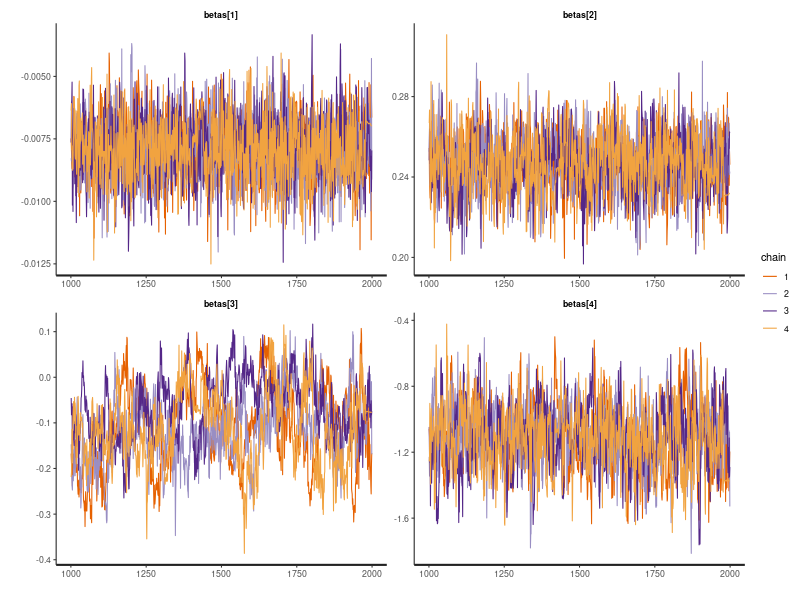
\includegraphics[height=75mm]{traceplot_betas.png}
  \caption{$\vec{\beta}$ Traceplots}
  \label{fig:tbetas}
\end{figure}

\begin{figure}[h!] 
	\centering
  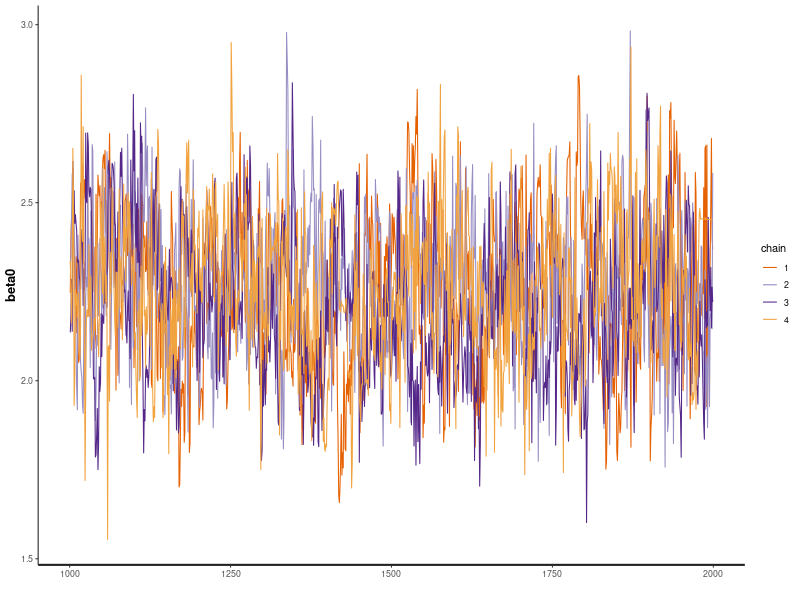
\includegraphics[height=75mm]{traceplot_beta0.png}
  \caption{$\beta_0$ Traceplot}
  \label{fig:tbeta0}
\end{figure}

\begin{figure}[h!] 
	\centering
  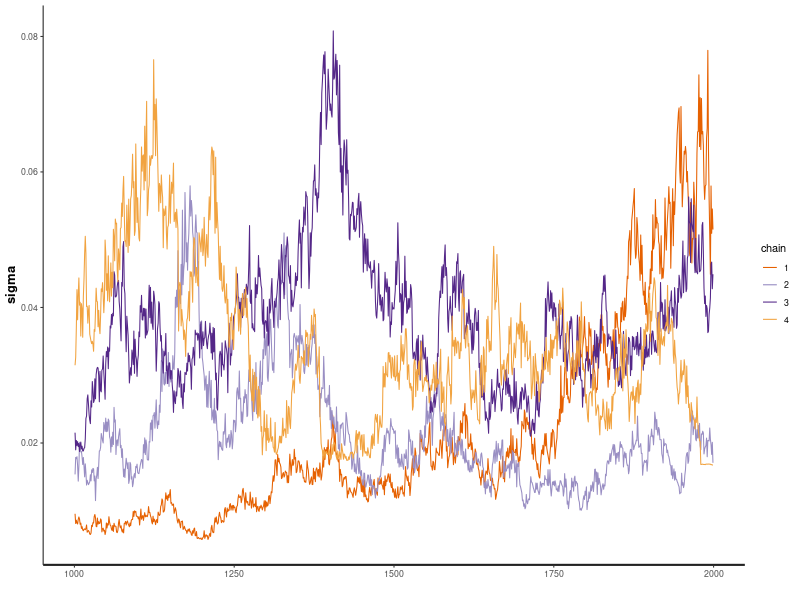
\includegraphics[height=75mm]{traceplot_sigma.png}
  \caption{$\sigma$ Traceplot}
  \label{fig:tsigma}
\end{figure}

\begin{figure}[h!] 
	\centering
  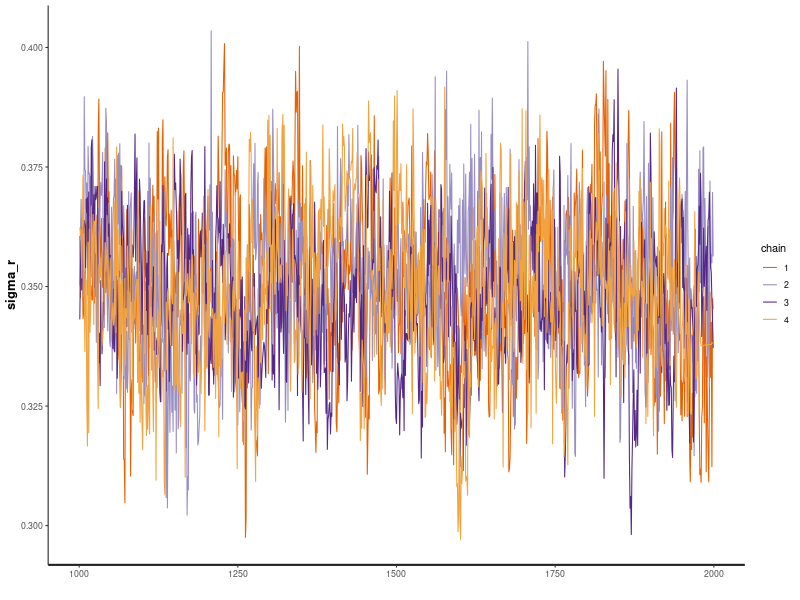
\includegraphics[height=75mm]{traceplot_sigma_r.png}
  \caption{$\sigma_r$ Traceplot}
  \label{fig:tsigma_r}
\end{figure}

\begin{figure}[h!] 
	\centering
  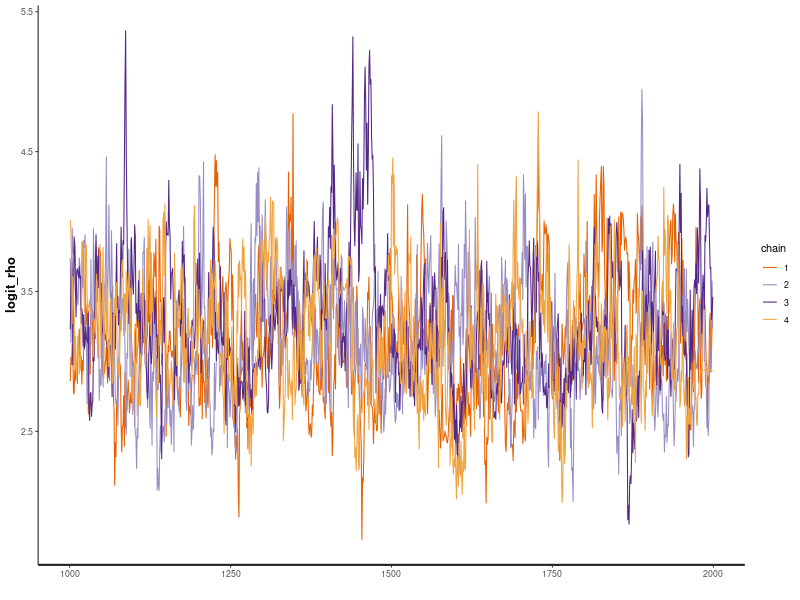
\includegraphics[height=75mm]{traceplot_logit_rho.png}
  \caption{$r$ Traceplot}
  \label{fig:tlogit_rho}
\end{figure}




\begin{figure}[h!] 
	\centering
  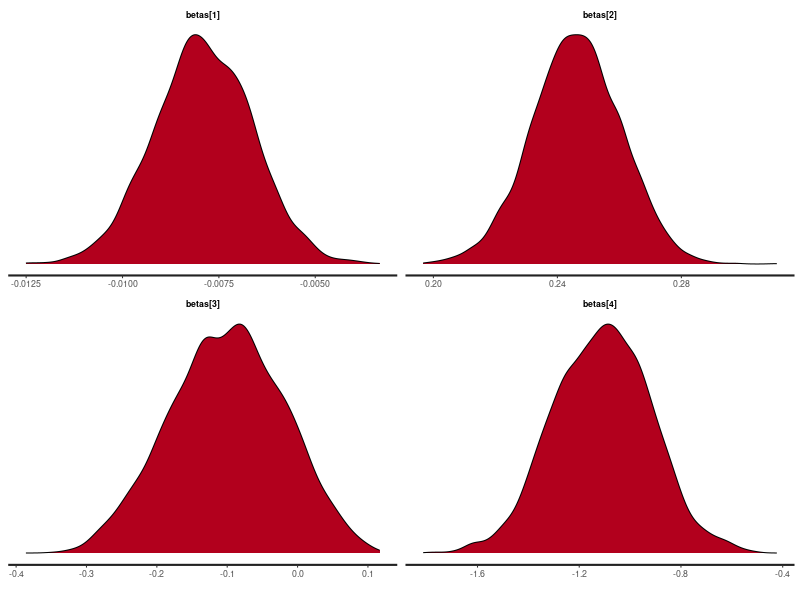
\includegraphics[height=75mm]{density_betas.png}
  \caption{$\vec{\beta}$ Densities}
  \label{fig:dbetas}
\end{figure}

\begin{figure}[h!] 
	\centering
  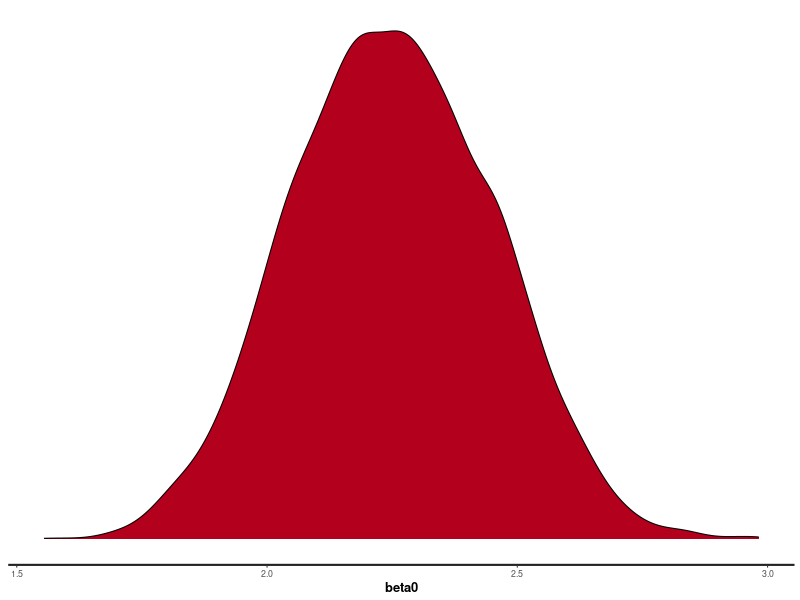
\includegraphics[height=75mm]{density_beta0.png}
  \caption{$\beta_0$ Density}
  \label{fig:dbeta0}
\end{figure}

\begin{figure}[h!] 
	\centering
  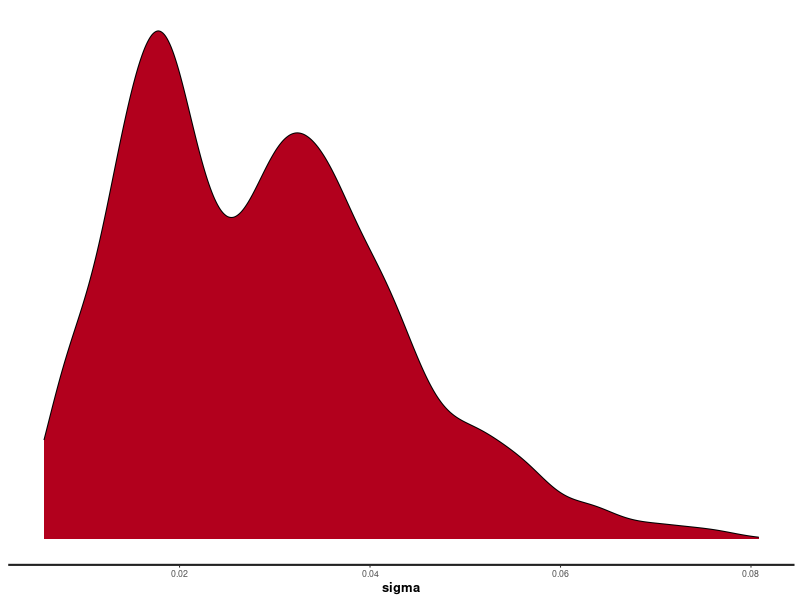
\includegraphics[height=75mm]{density_sigma.png}
  \caption{$\sigma$ Density}
  \label{fig:dsigma}
\end{figure}

\begin{figure}[h!] 
	\centering
  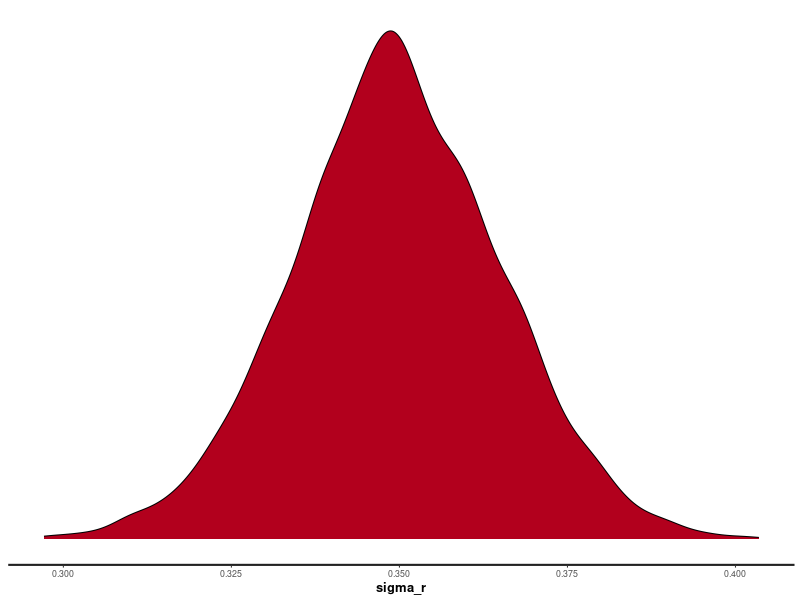
\includegraphics[height=75mm]{density_sigma_r.png}
  \caption{$\sigma_r$ Density}
  \label{fig:dsigma_r}
\end{figure}

\begin{figure}[h!] 
	\centering
  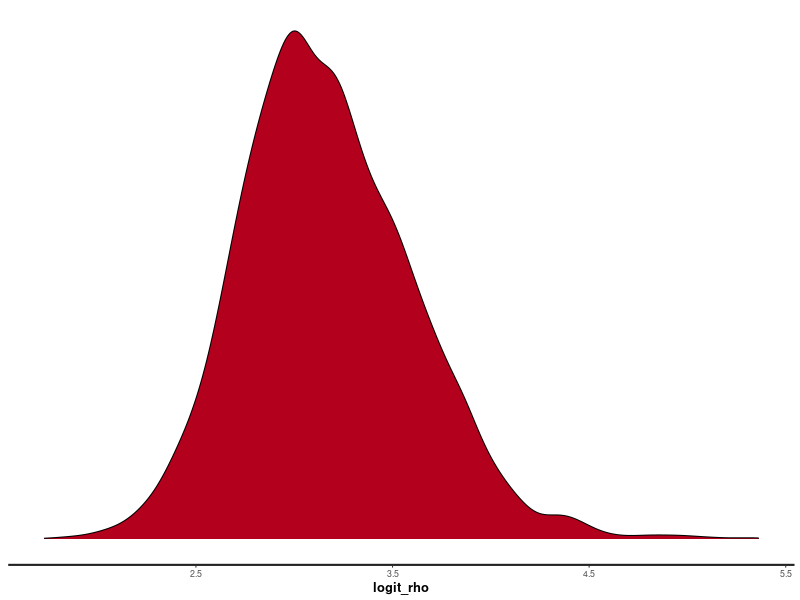
\includegraphics[height=75mm]{density_logit_rho.png}
  \caption{$r$ Density}
  \label{fig:dlogit_rho}
\end{figure}












\newpage
\bibliographystyle{apalike}
\bibliography{reference}
\end{document}